\documentclass[12pt,titlepage,figuresatend]{article}
%\usepackage[final]{JMR}
\usepackage{JMR}

\usepackage{authblk}
\renewcommand\Affilfont{\small}
%\renewcommand\Authands{, and }

\usepackage{lineno}
\linenumbers

\title{High-frequency variability in the\authorcr North Icelandic Jet}
%\author{First author\footnote{Address and email of first author} and Second Author\footnote{Address and email of second author}}
%\author[1]{First Author}
%\author[1]{Second Author}
%\author[1]{Third Author}
%\author[2]{Fourth Author}
%\affil[1]{Address of first author,\authorcr in two lines}
%\affil[2]{Address of second author in one lines}


\author{B. E. Harden\footnote{Woods Hole Oceanographic Institution, 266 Woods Hole Road, Woods Hole, MA 02543. bharden@whoi.edu}}
\author{R. S. Pickart}
%\author[2]{H\'{e}{\dh}inn Valdimarsson}
%\author[3]{Kjetil V{\aa}ge}
%\author[4,5]{Laura de Steur}
%\author[2,6]{Steingr\'{i}mur J\'{o}nsson}

\affil{Woods Hole Oceanographic Institution, Woods Hole, USA}
%\affil[2]{Marine Research Institute, Reykjavik, Iceland}
%\affil[3]{Geophysical Institute and Bjerknes Centre for Climate Research, \authorcr University of Bergen, Norway} 
%\affil[4]{Royal Netherlands Institute for Sea Research NIOZ, Texel, The Netherlands}
%\affil[5]{Norwegian Polar Institute, Troms{\o}, Norway}
%\affil[6]{University of Akureyri, Iceland}

\date{\today}

\begin{document}
\maketitle

\begin{abstract}
We describe the high-frequency variability in the North Icelandic Jet on the Iceland Slope using data from the densely instrumented K\"{o}gur mooring array deployed upstream of the Denmark Strait sill from September 2011 to July 2012. Significant sub-8-day variability is ubiquitous in all moorings from the Iceland slope with a dominant period of 3.6 days. We attribute this variability to Topographic Rossby Waves on the Iceland slope with a wavelength of 62 $\pm$ 3 km and a phase velocity of 17.3 $\pm$ 0.8 km$\,$day$^{-1}$ directed downslope (-9$^{\circ}$T). We test the theoretic dispersion relation for these waves against our observations and find good agreement between the direction of phase propagation. We additionally calculate a theoretical group velocity of 36 km$\,$day$^{-1}$ directed almost directly up-slope (138$\,^{\circ}$T) which agrees well with the propagation speed and direction of observed energy pulses. We use a wave tracing model to show that this wave energy is generated locally, offshore of the array, and not in the upstream or downstream directions. We hypothesize that either the meandering Separated East Greenland Current at the foot of the Iceland slope or intermittent aspiration into the Denmark Striat Overflow are the drivers of the Topographic Rossby Waves. Regardless of the formation mechanism, the waves appear to be a local phenomena, not found in an instrumented record upstream.

\end{abstract}

\section{Introduction}

The Denmark Strait Overflow is the major pathway of dense water out of the Nordic Seas. It transports 3.2 Sv, or approximately 50\%, of the total outflow \cite[]{Dickson1994,Jochumsen2017}, and hence plays a crucial role in the Atlantic meridional overturning circulation (AMOC). While the existence of this overflow has been known for many decades, our understanding of the processes that govern it and the underlying dynamics remains incomplete. One important aspect that requires further study is determining the upstream sources of the dense water and how it approaches the sill. If we are to determine how a changing climate might impact the AMOC, we need to understand better the connection between the water mass transformation process and the flux of newly ventilated water to Denmark Strait. 

Most of the Denmark Strait Overflow water (approximately 70\%) comes from the East Greenland Current by way of the Nordic Seas boundary current system \cite[]{Vage2013,Harden2016} (see Figure \ref{mainmap}). Specifically, warm Atlantic inflow across the Greenland-Scotland Ridge is progressively cooled as it flows northward towards Fram Strait, much of it recirculating in the strait and subducting to mid-depth \citep[]{Mauritzen1996}. This is joined by Atlantic water exiting the strait that has circumnavigated the Arctic, and together the transformed Atlantic water flows southward in the East Greenland Current.  As the current rounds Scoresby Sund, it splits into two branches (Figure \ref{mainmap}). One continues towards the sill as a shelfbreak jet \cite[]{Havik2017}. The other carries approximately 60\% of the East Greenland Current water out into the central strait via eddies and/or gyre-like deflections of the shelfbreak jet \cite[]{Vage2013,Harden2016}. This separated pathway then flows into the strait along the outer Iceland slope. 


\begin{figure}[p!]
  \centering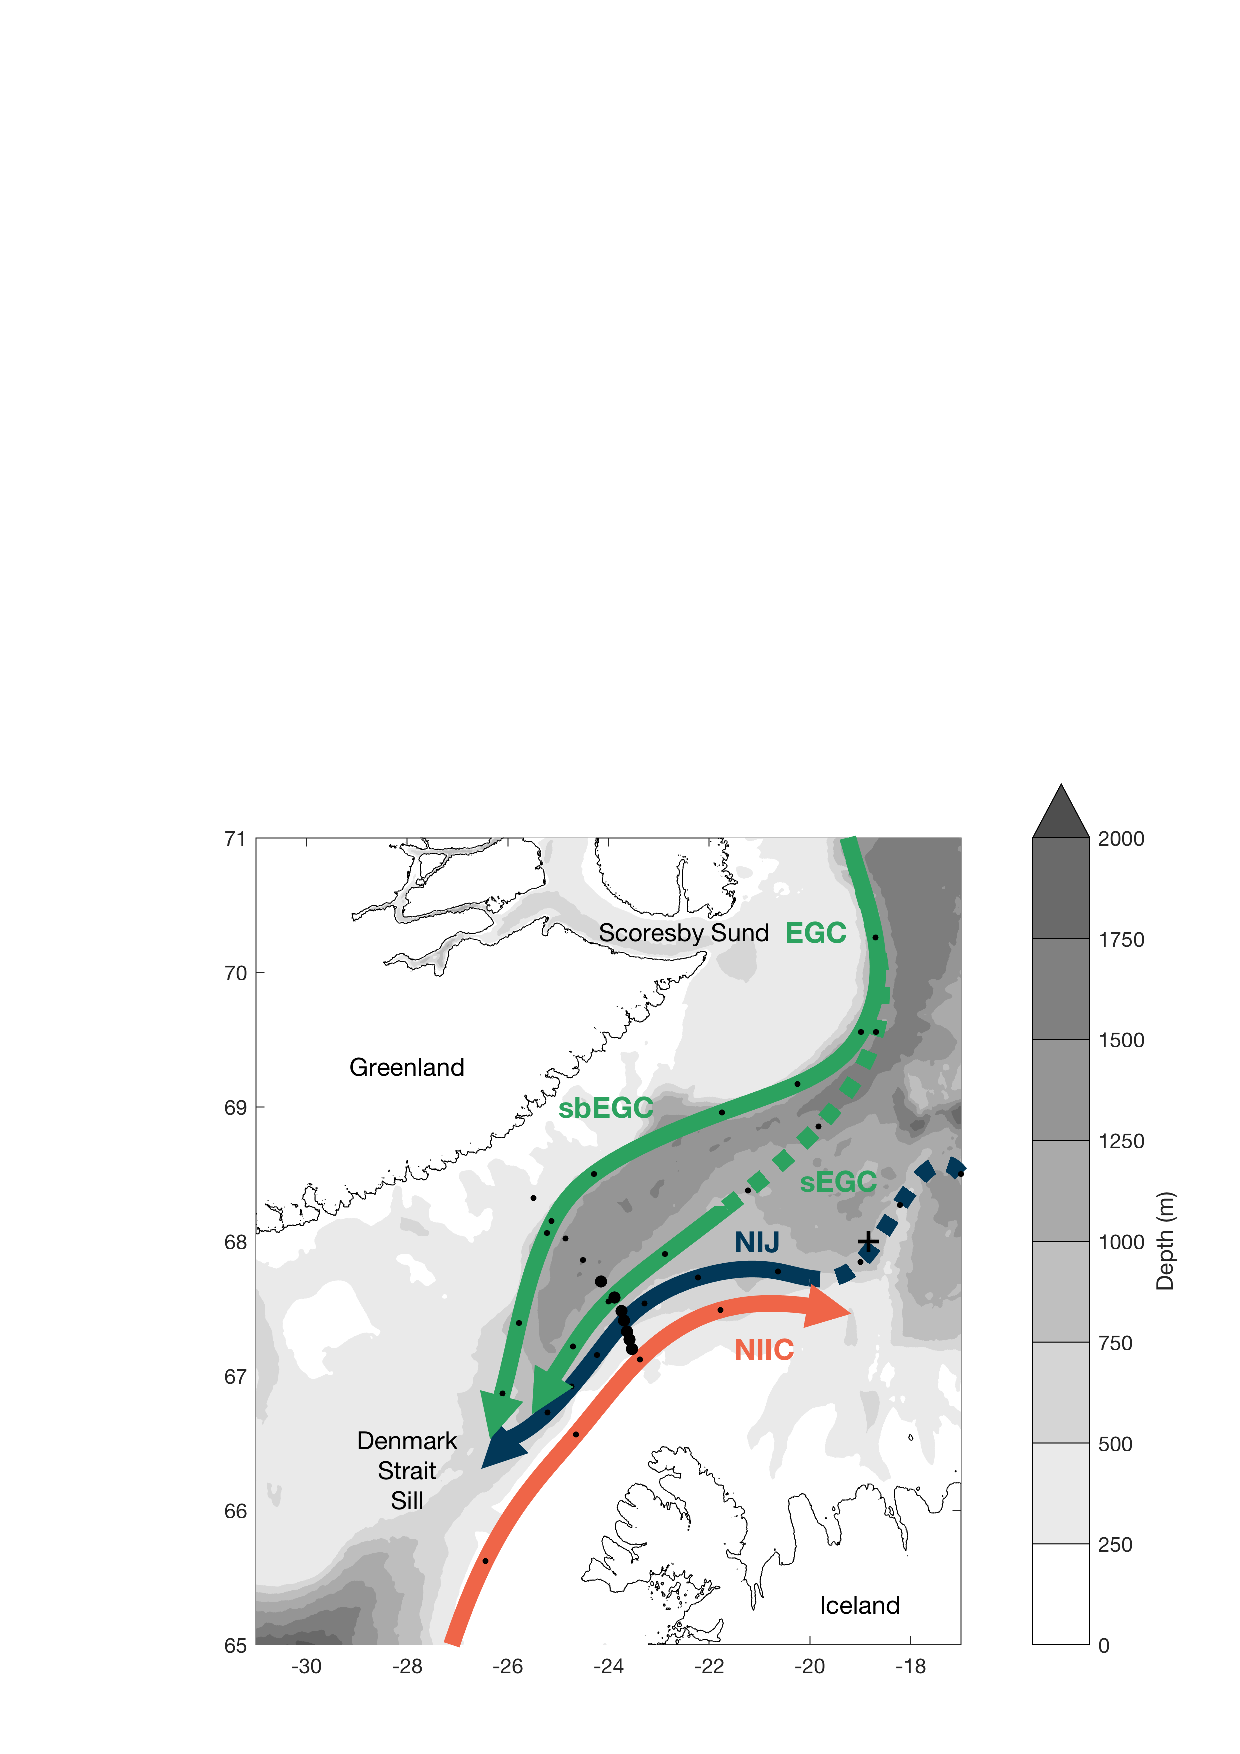
\includegraphics[width=\hsize]{./figures/mainmap.pdf}
  \caption{Map of the study region showing the overflow pathways approaching the Denmark Strait Sill: the North Icelandic Jet (NIJ) and the two East Greenland Current (EGC) pathways, one along the shelfbreak (sbEGC) and the other in a separated branch on the Iceland Slope (sEGC). Dashed portions show parts of pathways that still need further clarification. Also shown is the northward flowing surface-intensified current, the North Icelandic Irminger Current (NIIC). Black dots show the locations of the moorings in the K\"{o}gur array with larger dots indicating the subset of seven moorings used in this study. The upstream cross is the mooring to the west of the Kolbensey ridge referred to in the text. The bathymetry is from IBCAO v3.}{\label{mainmap}}
\end{figure}

The remaining 30\% of Denmark Strait Overflow water is supplied by the North Icelandic Jet (NIJ), a more recently discovered branch of the upstream circulation \cite[]{Steingrimur2004,Vage2011}. This mid-depth intensified jet advects waters distinct from those found in the East Greenland Current (colder and fresher) suggestive of a source in the central Iceland or Greenland seas \cite[]{Vage2011,Vage2015,Harden2016}. The NIJ contains the densest water that feeds the overflow; its waters are found in the deepest part of the sill \cite[]{Mastropole2017} and subsequently sink to the deepest depths in the core of the overflow.

The leading hypothesis for the formation of the NIJ, supported by both models and observations, is that it represents the lower limb of a local overturning cell in the Iceland sea \cite[]{Vage2011,Behrens2017}. The upper limb of the cell is the NIIC, which sheds warm water into the Iceland Sea that is cooled by air-sea heat loss. The transformed water then returns southward towards the boundary where it sinks and forms the NIJ. However, many questions remain unanswered about this proposed system. For instance, the winter mixed-layers in the Iceland Sea don't appear to be dense enough to account for the deepest water in the NIJ \cite[]{Vage2015}, whereas those in the Greenland Sea do \cite[]{Strass1993,Rudels2002}.

Regardless of the source of the NIJ, it clearly constitutes a vital component of the circulation upstream of the sill. \cite{Harden2016} investigated the jet's mean and seasonal contribution to the overflow, demonstrating that there is time-dependent partitioning of transport between the NIJ and the other two overflow branches on weekly to monthly timescales, likely driven by the wind. \cite{Pickart2017} noted that the NIJ appears to be coupled to the northward-flowing NIIC and that, on occasion, it consists of multiple branches. Using historical hydrographic data, \cite{Pickart2017} also revealed a clear link between the interannually varying properties of the NIJ and those of the densest water at the Denmark Strait sill, leaving little doubt that the NIJ is a major source of the overflow plume. 

It has long been known that the Denmark Strait Overflow varies on short (order days) timescales \cite[]{Smith1976,Bruce1995,Kase2003}. Some of this variability is associated with the passage of lenses of cold, dense, overflow water referred to as boluses \cite[]{Cooper1955}. Recently, \cite{Appen2017} identified a second type of mesoscale feature in the strait that was termed a pulse. In contrast to boluses, pulses correspond to a thinning of the overflow layer associated with a large increase in equatorward velocity. Both of these features have been identified in a high-resolution regional model as well \cite[]{Almansi2017}. \cite{Appen2017} showed that, between boluses and pulses, a mesoscale feature passes through Denmark Strait on average every 2 days. Presently, however, it is unknown if these disturbances originate from upstream or if they are associated with local dynamics near the sill. 

The goal of the present study is to shed light on some of the above processes by describing the high frequency variability of the NIJ north of the Denmark Strait. We use timeseries data from a year-long mooring array that was maintained roughly 200~km upstream of the sill (Figure \ref{mainmap}). This is the same data set used by \cite{Harden2016} to investigate the mean and seasonal attributes of the NIJ. While \cite{Harden2016} mentioned that the NIJ exhibits high-frequency variability, they did not elaborate. We begin with a brief description of the data, followed by a characterization of the high-frequency signal. We discuss how this signal is consistent with the existence of Topographic Rossby waves on the Iceland slope and go on to investigate the source region of the energy in these waves through inverse wave tracing.


\section{Data and Methods}

The data for this study come from the densely instrumented K\"{o}gur mooring array spanning the Denmark Strait approximately 200 km upstream of the sill. The array was deployed for 11 months from September 2011 to July 2012 and consisted of 12 moorings (named KGA 1-12) equipped with instrumentation to measure both the hydrography and velocity of the water column from 50 m to the bottom. \cite{Harden2016} present a detailed description of the mooring data, including the instrumentation, processing steps, and sensor accuracies. The array captured the majority of the overflow water (denser than 27.8 kg$\,$m$^{-3}$) passing through the northern part of the strait towards the sill.

\begin{figure}[p!]
  \centering\includegraphics[width=.9\hsize]{./figures/plot_section.pdf}
  \caption{Mean vertical section of the along-stream (cross-transect) velocity (top), and median sections of potential temperature (middle) and salinity (bottom) for the 11-month period of the K\"{o}gur array. Overlaid in black contours on each panel is the mean density with the 27.8 kg$\,$m$^{-3}$ isopycnal (the upper boundary of Denmark Strait Overflow Water) highlighted. The viewer is looking to the northeast with Iceland on the right. Positive velocities are equatorward. The horizontal black dashed line indicates the depth of the Denmark Strait sill. The moorings (black triangles) are labeled, and the 
  average instrument locations are shown by the grey points. The bathymetry is from a shipboard echosounder.}{\label{fig_section}}
\end{figure}

Here we use primarily the gridded product described in \cite{Harden2016}, which has a lateral resolution of 8km and vertical resolution of 50 m. Because of our focus on the Iceland slope, we consider a subset of these data up to and including the location of mooring KGA 7, approximately 70 km offshore of the Iceland shelfbreak. The mean velocity sections demonstrate that this portion of the array captures both the NIJ and the majority of the Separated EGC (Figure \ref{fig_section}). For parts of the analysis we also use the data on a mooring-by-mooring basis. All of the velocities have been de-tided using a 36-hour low-pass filter.

Additional data come from a mooring located approximately 200 km upstream of the K\"{o}gur Array on the west side of the Kolbesney Ridge (68$^{\circ}$00'N, 18$^{\circ}$50'W, see Figure \ref{mainmap}) This was deployed on the 1000 m isobath from September 2007 to mid-October 2008 and consisted of a McLane Moored Profiler and acoustic current meter providing profiles between 100~m and the bottom at 8 hour intervals. As with the K\"{o}gur data, we low-passed the velocity timeseries using a 36-hr filter to remove the tidal components of the flow. These data are described in greater detail by \cite{Jonsson2012}.

The inverse wave tracing of topographic Rossby waves (TRWs) was done using the model described by \cite{Meinen1993} and implemented by \cite{Pickart1995} for investigating TRWs in the Deep Western Boundary Current off of Cape Hatteras, North Carolina. The method uses the TRW dispersion relation to calculate the group velocity and then backtracks the evolution of the wave with a time step of 30~minutes. The wave parameters are recalculated at each step for the local bottom depth, bottom slope, and water column stratification. A new group velocity is then found and used to further trace the wave. Most of the required input parameters for the inverse wave tracing model come directly from the moored data and are the same as those used for the theoretical TRW dispersion relation calculations (see Section \ref{results}.\ref{TRWsec}.). For the bathymetry we used the International Bathymetric Chart of the Arctic Ocean 30-arcsec gridded product \cite[]{Jakobsson2012}. To remove seamounts and other sharp topographic features we smoothed the bathymetry using a filter of 60 km (comparable to our measured TRW wavelength). In contrast to \cite{Pickart1995} who subsequently fit splines to the data to be able to find the bottom depth and gradients at any location, we deemed our resolution to be high enough (and our smoothing window great enough) to simply use linear interpolation. The total integration period for the wave tracing was 48 hours.


\section{Results}
\label{results}

As discussed in \cite{Harden2016}, the vertical sections of velocity and hydrography at the K\"{o}gur site show the signatures of both the NIJ and the Separated EGC. However, the two features are merged to some degree in the mean (Figure \ref{fig_section}). The NIJ is on the upper Iceland slope and is characterized by a mid-depth intensified flow carrying the coldest, densest overflow water banked up on the slope. The Separated EGC is farther offshore; its key features are a surface intensification and the transport of warmer, saltier overflow water at approximately 300 m. Inshore of both these currents, on the Iceland shelf, is the poleward flowing NIIC (see also Figure \ref{mainmap}).


\begin{figure}[p!]
  \centering\includegraphics[width=\hsize]{./figures/hoff_vars.pdf}
  \caption{Hovm\"{o}ller plots from the gridded mooring data of a) the depth-mean along-stream velocity (below 100 m, same for all plots); b) the 8-day high-passed, depth-mean component of velocity in the direction of the major axis of the local variance ellipse; and c) the wavelet amplitude at a 4-day period for the depth-mean velocity. Iceland is to the right of each panel as in Figure \ref{fig_section} The wavelet analysis uses the jLab toolbox \cite[]{Lilly2017} with standard Morlet wavelets with $\gamma$=3 and $\beta$ = 2. The sloped, black guidelines in panel c are angled at the theoretical group velocity for the measured topographic Rossby waves (see text for details).}{\label{fig_hoff}}
\end{figure}


The two overflow currents are merged in the mean largely due to the high degree of variability on weekly timescales. The depth-integrated, along-stream velocity exhibits constant pulsing through this portion of the strait (Figure \ref{fig_hoff}a). The period of the pulsing in the vicinity of the NIJ is concentrated at sub-8-day periods with a maximum average energy at 3.6 days (Figure \ref{fig_waveSpec}). Farther offshore, near the Separated EGC, we also see such short-period pulses in addition to more consistent longer-period variability (Figure \ref{fig_hoff}a). The lower frequency signals were described by \cite{Harden2016} and attributed in part to the time-varying upstream bifurcation of the EGC. Here we focus on the higher-frequency, sub-8-day variability. To facilitate this we used an 8-day butterworth filter.\footnote{Different period filters were implemented, ranging in length from 4 days to 30 days, but the 8-day filter was most effective in isolating the peak high-frequency energy.}

\begin{figure}[ht!]
  \centering\includegraphics[width=\hsize]{./figures/TRWwavelet.pdf}
  \caption{Top: Depth-averaged along-stream (black) and cross-stream (grey) components of velocity for the grid point closest to mooring KGA 3. Bottom left: Wavelet spectrum of the depth-averaged velocity using Morlet wavelets \cite[]{Lilly2017}. The color scale for this plot is at the top right. Bottom right: Mean wavelet amplitude for the length of the deployment. The dashed line in the bottom panels indicates the 8-day cut-off period for the high-pass filter used in this study.}{\label{fig_waveSpec}}
\end{figure}

The variance ellipses of this high-frequency variability for each mooring are useful for characterizing different regimes across the array (Figure \ref{fig_ellipse}). In the NIIC (KGA 1), the variance ellipse is elongated in the direction of the mean flow indicative of a current pulsing along its axis. By contrast, within the Separated EGC (KGA 6 and 7), the elongation of the variance ellipses is perpendicular to the mean flow demonstrating that this current meanders. However, in the NIJ (KGA 2-4), the major axes of the variance ellipses are aligned at an oblique angle to both the mean flow and the underlying bathymetry. KGA 5 appears to be in a transition region between conditions in the NIJ and those in the Separated EGC.


\subsection{Topographic Rossby Waves}
\label{TRWsec}

We resolved the sub-8-day depth-averaged flow in the gridded product along the major axis of the variance ellipses at each offshore location. Particularly in the NIJ, the variability along these axes have a sinusoidal form and are lagged between moorings such that the pulses of current progress offshore in time (Figure \ref{fig_hoff}b). This implies a downslope phase propagation of this variability.

We argue that this is the signature of TRWs. These waves are supported by topographic $\beta$ and result in transverse fluctuations that are often at an oblique angle to the mean flow. TRWs are found in many slope regions of the world’s oceans \cite[]{Garrett1979,Louis1982,Pickart1990}. Key features of TRWs include wave vectors (and hence phase velocities) that are perpendicular to the velocity variability, a group velocity which is at an oblique angle to the phase velocity, and a tendency to be bottom-trapped in regions of significant stratification.

\begin{figure}[ht!]
  \centering\includegraphics[width=\hsize]{./figures/map_ellipse.pdf}
  \caption{Aspects of the flow measured by the K\"{o}gur moorings (black circles). The thin vectors indicate the mean velocity averaged from 100 m to the depth of the ADCP at each mooring (see gray lines in Figure \ref{fig_section}). Also shown are the 8-day high-passed variance ellipses for the same depth range. The thick black arrow ($C_{p}$) denotes the direction of TRW phase propagation averaged over KGA 2-4 (plotted at KGA 3). The dashed black arrow shows the direction of TRW group velocity ($C_{g}$). All vectors and variance ellipses are drawn to the same scale as indicated. The long black line is the mean downslop direction averaged between KGA 2-4. Bathymetry is from IBCAO v3.}{\label{fig_ellipse}}
\end{figure}

Given that the phase propagation is perpendicular to the velocity variability, we deduce that the wave phase is progressing downslope at -9$^{\circ}$T (average from moorings KGA 2--4, see Figure \ref{fig_ellipse}). Following \cite{Pickart1990}, we then calculated the phase speed over the range of moorings KGA 2--4 (where the wave signal is most pronounced) using,

\begin{eqnarray*}
  c_p = \frac{1}{T}\, \frac{360}{\overline{\phi}}\, \frac{\overline{\Delta S}}{cos(\Delta)}
\end{eqnarray*}

where $T$ is the wave period (= 3.6 days), $\overline{\phi}$ is the average phase offset (= 48 $\pm$ 3$\,^{\circ}$), $\Delta S$ is the average instrument spacing (= 8.1 $\pm$ 0.2$\,$km), and $\Delta$ is the angle between the mooring array and the direction of wave propagation (= 8 $\pm$ 4$\,^{\circ}$). The resulting phase speed is 17.3 $\pm$ 0.8 km$\,$day$^{-1}$ corresponding to a wavelength of 62 $\pm$ 3 km. The error estimates arise in equal contributions from uncertainties in $\overline{\phi}$, $\Delta S$, and $\Delta$.

As a consistency check that the observed fluctuations are in fact TRWs, we can employ the TRW dispersion relation for a uniformly stratified ocean neglecting planetary $\beta$. Following \cite{Pedlosky1979}, this can be written as:

\begin{eqnarray*}
  T = \frac{2\pi \,tanh(\frac{2\pi ND}{\lambda f})}{N\Gamma sin(\theta)}\\
\end{eqnarray*}

where $T$ is the period of the wave, $N$ is the average water column Brunt V{\"a}is{\"a}l{\"a} frequency (= 3.3 x 10$^{-5}$, averaged using the gridded data below 100 m), $D$ is the depth (= 500 m), $\lambda$ is the wavelength, $f$ is the Coriolis parameter (= 1.35 x 10$^{-4}$), $\Gamma$ is the bottom slope (= 0.016, from IBCAO v3), and $\theta$ is the phase velocity direction relative to downslope.

We can test the predicted value of $\theta$ against the observed value using our knowledge of the other variables. The predicted angle of 29$\,^{\circ}$ compares well with the measured value of 24$\,^{\circ}$ (from the average downslope angle between moorings KGA 2--4). There is of course uncertainty in the measured downslope angle depending on the region selected for the averaging. For example, if we expand the calculation of the downslope direction to encompass KGA 1--5, the measured $\theta$ becomes 33$\,^{\circ}$, which still agrees well with the predicted value. In addition, the bottom-trapping scale (=$f/N\,k$) is much greater than 1000 m, in agreement with the observed velocities which are largely barotropic. 

All of this supports our assertion that the dominant high-frequency variability in the NIJ is due to TRWs. The obvious question is, where and how are these waves being generated? Using the dispersion relation we can calculate the group velocity. For the observed parameters, we find this to be 36 km$\,$day$^{-1}$ directed almost directly up-slope at the array site (138$\,^{\circ}$T, see Figure \ref{fig_ellipse}). This implies that the energy source lies offshore. We can corroborate this onshore propagation of energy observationally by considering the wavelet amplitude for the 4-day signal at each mooring site. The Hovm\"{o}ller plot of this shows clear occurrences of onshore energy propagation that are in line with the predicted group velocity (Figure \ref{fig_hoff}c). 

\subsection{Wave Tracing and TRW Formation Mechanisms}

In order to shed light on the source of the TRWs, we implemented the inverse wave tracing model described in Section 2. In particular, we calculated the wave paths backwards in time from moorings KGA 2--5. For each mooring, the model was initialized with the local wavenumber (assuming constant phase velocity and wave period). Since KGA 5 only marginally displayed TRW behavior, the results from that mooring should be considered less robust. The calculated paths indicate that the waves originate offshore of the moorings in the vicinity of the deep Blosseville Basin (Figure \ref{fig_waveTrace}). While the traces diverge somewhat going offshore, it is clear that they do not deflect significantly upstream or downstream. In other words, the energy is not propagating along the Iceland continental slope.

\begin{figure}[p!]
  \centering\includegraphics[width=\hsize]{./figures/wave_trace.pdf}
  \caption{Paths of the Topographic Rossby Waves (thin lines) computed using the inverse wave tracing model for moorings KGA 2-5. Wave traces are truncated as they pass the 1500 m isobath. The bathymetry is from IBCAO v3 smoothed over 60 km (see text for details).}{\label{fig_waveTrace}}
\end{figure}

TRWs are a ubiquitous feature in the middle Atlantic Bight between Cape Hatteras, NC and the Grand Banks \cite[]{Louis1982,Johns1986,Pickart1990}. The source of the waves appears to be the Gulf Stream. Both \cite{Hogg1981} and \cite{Schultz1987} argued that TRWs observed along the US continental slope emanated from large amplitude Gulf Stream meanders offshore. \cite{Louis1982} made the case that bursts of TRWs measured south of Nova Scotia resulted from Gulf Stream eddy formation. \cite{Pickart1995} demonstrated that the TRWs observed near Cape Hatteras were forced by meanders of the Gulf Stream as it flowed over a bend in topography farther to the east. 

In light of these studies, it is natural to suspect that the TRWs measured at the K\"{o}gur array site are generated by the Separated EGC. This current is energetic, and, as noted above, is subject to significant meandering (akin to the Gulf Stream). The wave tracing indicates that the energy emanates from the Blosseville Basin where the Separated EGC resides. Additionally, there is evidence that times of strong TRW activity on the upper slope are often preceded slightly by increases in meander energy offshore (Figure \ref{fig_hoff}). The high-energy event in November is one example of this, but there are additional instances in late October, late December, and early March. 

Another possible trigger for the waves is the intermittent aspiration of deeper waters towards the Denmark Strait Sill. \cite{Harden2016} demonstrated that 0.6 Sv of the overflow transport approaching the sill does so from below sill depth. Pulsing of this aspirated component of the flow across the isobaths could initiate topographic wave activity. Regardless of the mechanism, the presence of TRWs raises the question of whether they are present along the entire Iceland slope or whether they are unique to our sampling region. To address this we examined the velocity data from a mooring deployed approximately 200 km upstream on the Iceland slope near the Kolbeinsey ridge from 2007--2008 \cite[]{Jonsson2012}. The depth-mean velocity showed very little energy in the 4-day period, at odds with the large TRW signal found at this period at the K\"{o}gur array. Notably, the upstream mooring site is quite far from the Separated EGC (Figure \ref{mainmap}) and hence lacks that as an energy source. 


\section{Summary and Discussion}

We have documented the existence of energetic Topographic Rossby Waves (TRWs) within the North Icelandic Jet (NIJ) using observations from the densely-instrumented K\"{o}gur Array located approximately 200 km upstream of the Denmark Strait Sill. The mean period of the waves is 3.6 days, the wavelength is 62 $\pm$ 3 km, and the phase velocity is 17.3 $\pm$ 0.8 km$\,$day$^{-1}$ directed downslope (-9$\,^{\circ}$T). Using the TRW dispersion relation, we corroborated our observed direction of phase propagation relative to the downslope direction (24$^{\circ}$) with the theoretical value (29$^{\circ}$). We further calculated that the wave energy is progressing up-slope (138$\,^{\circ}$T) at 36 km$\,$day$^{-1}$, in agreement with our observational data. It is likely that the energy in the TRWs emanates locally near the mooring site, either through the meandering of the offshore Separated East Greenland Current (EGC), or through pulses of cross-bathymetric flow due to the aspiration of deep overflow water as it approaches Denmark Strait. 

Notably, our data imply that the dominant high-frequency variability at the K\"{o}gur site does not originate from the Denmark Strait, nor does it propagate towards the sill. This is perhaps surprising in light of the fact that fluctuations of the dense overflow water at the sill occur on similar short timescales \cite[]{Jochumsen2017}. It suggests that the mesoscale features at the sill (boluses and pulses), diagnosed observationally by \cite{Appen2017} and in a model framework by \cite{Almansi2017}, are not triggered, nor directly trigger, the TRWs on the Iceland Slope. However, the likelihood of a connection between these features is still high given the geographic proximity and similarity in timescales, but is presumably mediated by another process. The Denmark Strait overflow is believed to be subject to hydraulic control \cite[]{Whitehead1998,Nikolopoulos2003}, and consequently, information should be transferred between upstream and sill variability, likely as Kelvin waves. The existence of any such connection and the impact on both the sill and NIJ variability requires more careful investigation and is the subject of an on-going study. 

Finally, one also needs to consider where the energy in the TRWs ends up and what impact it might have on the dynamics of the circulation inshore of the Iceland slope. The energy likely cascades into the North Icelandic Irminger Current (NIIC) where it dissipates, leading to enhanced mixing. It might also alter the stability of NIIC, which brings warm subtropical water into the Nordic Seas. \cite[]{Vage2011} hypothesize that the offshore flux of this warm water associated with the disintegration of the NIIC is tied to the overturning loop that forms the NIJ. Notably, eddies of NIIC water are found both in the Blosseville Basin \cite[]{Jonsson2012} and farther north in the Iceland Sea \cite[]{Vage2011}. It is intriguing to think that the TRWs described here could play a role in this aspect of the NIIC. 


\bigskip
\emph{Acknowledgments.}
We would like to thank the crew and technicians aboard the R/V Knorr and RSS James Clark Ross for the deployment and recovery of the K\"{o}gur moorings. This work was supported by National Science Foundation grants OCE-0959381 (BH and RP) and OCE-1558742 (RP). 


\bibliographystyle{JMR}
\bibliography{bib_master}

\end{document}
